\chapter{Range Minimum Queries}

Eine \term{range minimum Query}\index{range minimum query} gibt für ein array \( A \) (\( \left\vert A \right\vert \eqqcolon n \)) die Position des kleinsten Elements zwischen zwei Begrenzern \( 1 \leq l < r \leq n \) zurück:
\begin{equation*}
  \text{rmq}_A(l,r) = (\text{arg})\min_{l \leq k \leq r}A[k]
\end{equation*}

\begin{figure}[H]
  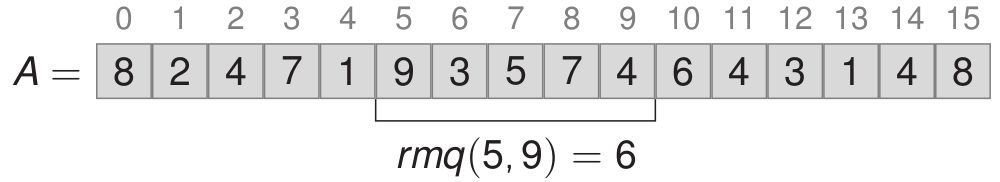
\includegraphics[width=0.6\textwidth]{rmqExample}
  \caption{Beispiel einer range minimum query}
\end{figure}

Ziel dieses Kapitels wird sein, einen Algorithmus anzugeben, mit dem eine RMQ-Abfrage in konstanter Zeit beantwortet werden kann, nachdem eine \( 2n + o(n) \) große Datenstruktur in Linearzeit vorbereitet wurde.

Ein naiver Ansatz, um eine range minimum query auszuführen, ist, einfach das Array zu durchlaufen und das Minimum zu speichern (und wenn nötig zu aktualisieren). Dafür ist keine Vorbereitungsarbeit nötig (also \( O(1) \)) und die Abfrage ist in \( O(n) \). Wir notieren
\begin{equation*}
  \left\langle O(1), O(n) \right\rangle\text{.}
\end{equation*}

\section{Lösung 1 --- \( \left\langle O(n), O(\log n) \right\rangle \)}

Baut man einen binären Suchbaum über das Array auf, so lässt sich die Komplexität der Abfrage auf \( O(\log n) \) reduzieren.

Hierzu betrachtet man die größtmöglichen Knoten, die vollständig im Abfrageintervall liegen (grün dargestellt), und berechnet das Minimum dieser.

\begin{figure}[H]
  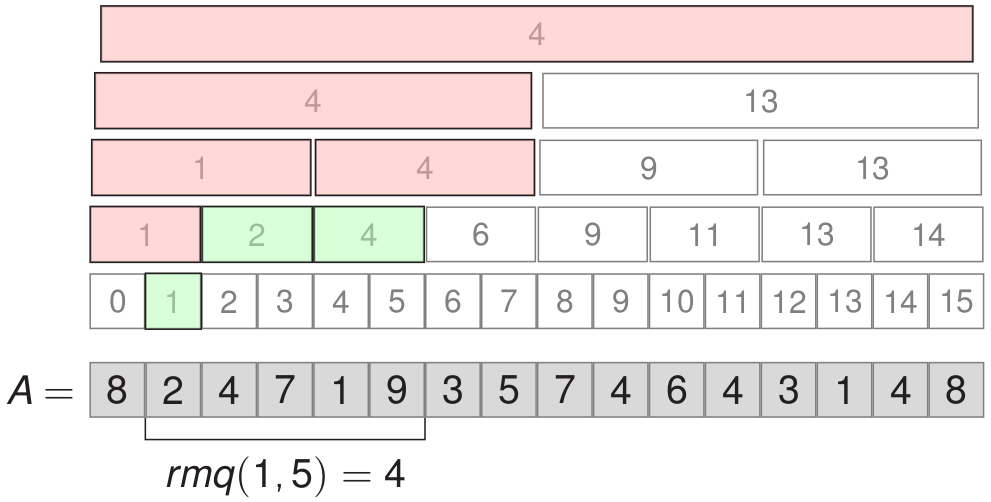
\includegraphics[width=0.6\textwidth]{rmqBST}
  \captionsetup{width=.7\textwidth}
  \caption{Die grauen Felder stellen die Knoten des binären Suchbaums dar, sie beinhalten die Position des Arrays, an der der Teilbaum, dessen Wurzel sie sind, den minimalen Wert annimmt. Die größten Knoten, die vollständig im Intervall liegen, sind grün markiert.}
\end{figure}

\section{Lösung 2 --- \( \left\langle O(n\log n),O(1) \right\rangle \)}

Wir reduzieren nun die Zeit, die zum Bearbeiten der rmq benötigt wird, auf \( O(1) \), indem wir für jedes \( A[i] \) ein Array \( M_i[0,\log n] \) vorberechnen. Es sei
\begin{equation*}
  M_i[j] = \text{rmq}_A(i,i+2^j-1)\text{.}
\end{equation*}

Idee ist es nun, \( \text{rmq}_A(l,r) \) aus der Überdeckung des Intervalls durch zwei Zweierpotenzen zu berechnen.

Wir suchen dafür \( 2^{\lfloor l - r \rfloor} \), also die größte Zweierpotenz, die kleiner ist als die Länge des Intervalls. Offensichtlich ist diese Zweierpotenz mehr als halb so groß wie das Intervall, also ist \( \text{rmq}_A(l,r) \) entweder das Minimum der ersten oder zweiten überdeckenden Zweierpotenz.

\begin{figure}[H]
  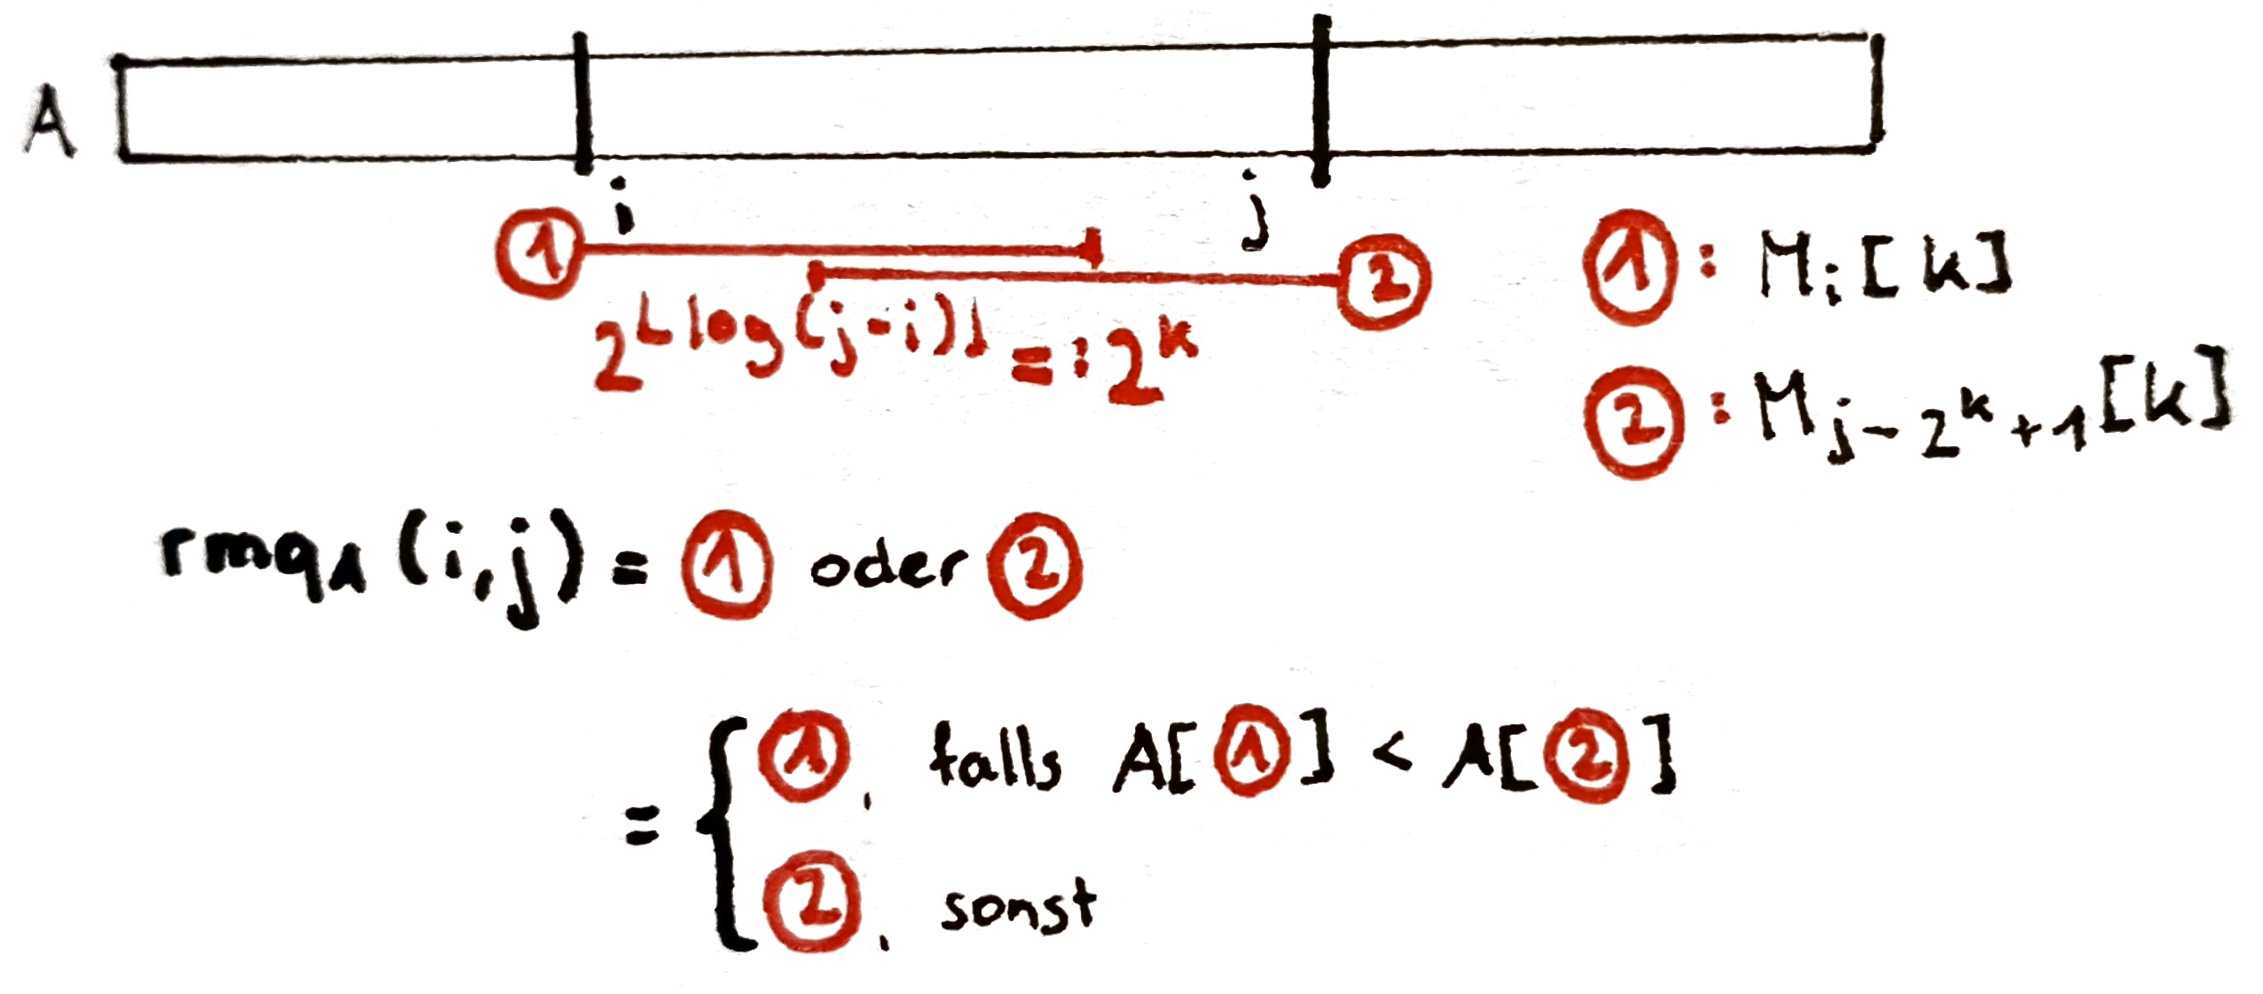
\includegraphics[width=0.5\textwidth]{rmqVersion2}
  \caption{Funktionsweise des zweiten rmq-Algorithmus}
\end{figure}

\section{Lösung 3 --- \( \left\langle O(n \log \log n), O(1) \right\rangle \)}

Wir wenden folgende Prozedur an:

\begin{enumerate}
  \item \( A \) in \( t = \frac{n}{\log n} \) Blöcke \( B_0, \dots, B_{t-1} \) der Größe \( \log n \) unterteilen.
  \item Array \( S[0,t-1] \) mit \( S[i] = \min\left \{ x \in B_i \right \} \) erstellen, rmq-Struktur nach Lösung 2 für \( S \) berechnen.
  \item Für jeden Block \( B_i \) rmq-Struktur nach Lösung 2 berechnen.
\end{enumerate}

Diese Prozedur liegt in \( O(n \log \log n) \).

Soll nun \( \text{rmq}_A(l,r) \) bestimmt werden, so geht das folgendermaßen:

\begin{enumerate}
  \item Bestimme die Blöcke \( l \in B_{l'} \) und \( r \in B_{r'} \).
  \item Berechne \( m = \text{rmq}_S(l'+1, r'-1) \). Wir nutzen also die Struktur über \( S \), um die rmq-Werte der Blöcke zwischen den beiden Grenzblöcken zu berechnen.
  \item Es seien \( k_0,k_1,k_2 \) die \( \text{rmq}_A \)-Resultate in den Blöcken \( l' \), \( r' \) und \( m \)
  \item \( \text{rmq}_A(l,r) = \text{arg}\min \left \{ A[k_0],A[k_1],A[k_2] \right \} \)\text{.}
\end{enumerate}

\section{Lösung 4 --- \( \left\langle O(n),O(1) \right\rangle \)}

Zur Konstruktion des Algorithmus mit linearem Platzverbrauch benötigen wir kartesische Bäume.

\subsection{Kartesischer Baum}

Der \term{kartesische Baum}\index{Kartesischer Baum} eines Arrays \( A \) ist folgendermaßen definiert:

\begin{itemize}
  \item \emph{Wurzel} des Baums ist das (linkste) kleinste Element \( m \) des Arrays, mit Position als Label.
  \item Die Wurzel hat zwei Kindknoten --- die Wurzel des linken und die Wurzel des rechten Subarrays von \( A \) (jeweils von \( m \) aus).
  \item Rekursion.
\end{itemize}

\subsection{Implementierung}

Die Implementierung funktioniert so:

\begin{enumerate}
  \item Partitioniere das Array in Blöcke der Größe \( s \) --- jeder Block entspricht einem kartesischen Baum.
  \item Berechne alle \( s^2 \) Möglichkeiten aller \( \frac{1}{s+1} \binom{2s}{s} \) möglichen kartesischen Bäume der Größe \( s \) in einer Tabelle \( P \). Diese benötigt \( O(2^{2s}s^2) \) Speicher, also braucht \( P \) für \( s = \frac{\log n}{4} \) nur \( o(n) \) Speicher.
  \item Berechne nach Lösung \( 2 \) die Struktur für das Array \( A' \), welche aus den blockweisen Minima von \( A \) besteht (\( O(n) \) Zeit, \( O(n) \) Platz).
\end{enumerate}

\section{Lowest Common Ancestor}

Gegeben sei ein Baum \( T \) mit Wurzel, \( \left\vert T \right\vert = n \). Es sei
\begin{equation*}
  \text{LCA}_T(v,w)
\end{equation*}
der \term{lowest common Ancestor}\index{lowest common ancestor} der Knoten \( v,w \) in \( T \), also der Knoten \( a \in T \), der
\begin{itemize}
  \item Vorgänger von \( v \) und \( w \) ist und
  \item maximalen Abstand zur Wurzel hat.
\end{itemize}

\begin{figure}[H]
  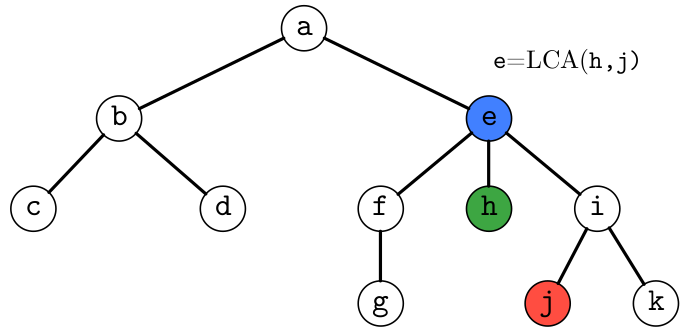
\includegraphics[width=0.5\textwidth]{LCA}
  \caption{lowest common ancestor der Knoten \( h \) und \( j \) ist \( e \)}
\end{figure}

\subsection{Von RMQ zu LCA}

\begin{lemma}
  Gibt es eine \( \left\langle f(n),g(n) \right\rangle \)-Lösung für RMQ, so gibt es eine Lösung in
  \begin{equation*}
    \left\langle f(2n-1)+O(n),g(2n-1)+O(1) \right\rangle
  \end{equation*}
  für LCA.
  \begin{proof}
    Sei
    \begin{itemize}
      \item \( T \) der kartesische Baum des Arrays \( A \),
      \item \( E[0,\dots,2n-2] \) das Knoten-Array, die in einer DFS-Euler-Tour von \( T \) besucht wurden,
      \item \( L[0,\dots,2n-2] \) die entsprechende Tiefe der Knoten in \( E \),
      \item \( R[0,\dots,n-1] \) ein Array mit \( R[i] = \min\left \{ j : E[j] = i \right \} \) für jeden Knoten \( i \in T \), also wo in der Euler-Tour der Knoten \( i \) das erste Mal auftaucht.
    \end{itemize}
    Dann ist
    \begin{equation*}
      \text{LCA}_T(v,w) = E[\text{RMQ}_L(\min\left \{ R[v],R[w] \right \}, \max\left \{ R[v],R[w] \right \})]\text{.}
    \end{equation*} \qed \\
    \begin{figure}[H]
      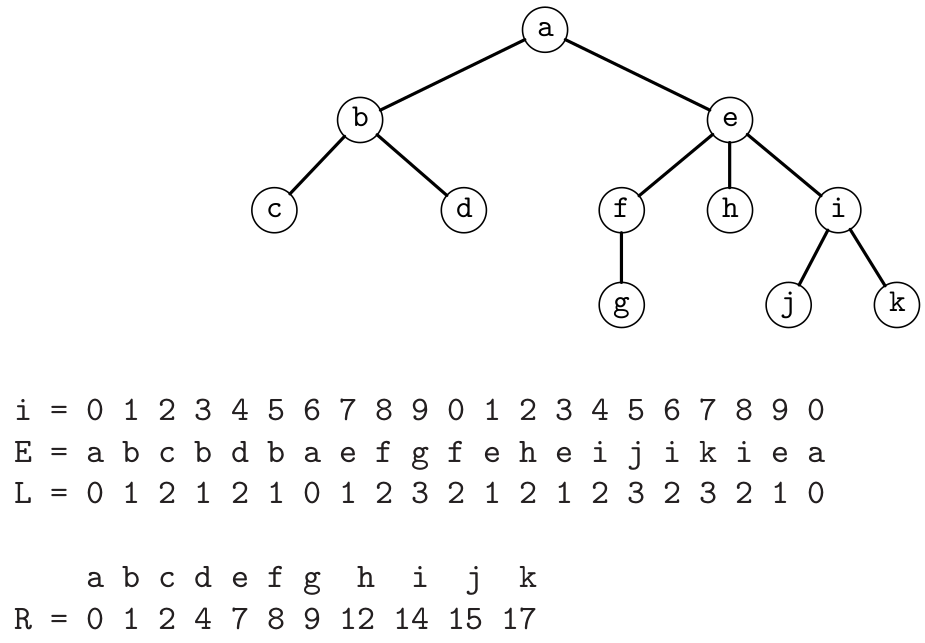
\includegraphics[width=0.6\textwidth]{LCAConstruction}
      \caption{Konstruktion der Hilfsarrays für LCA}
    \end{figure}
    \textcolor{red!80!black}{\textbf{Achtung}}: Die Tiefe zweier Knoten, die nacheinander bei der Euler-Tour besucht wurden, kann sich höchstens um 1 unterscheiden, also
    \begin{equation*}
      (L[i]-L[i+1]) \in \left \{ -1,1 \right \}\text{.}
    \end{equation*}
    Wir müssen also nur RMQs über Arrays lösen, bei denen sich zwei nacheinanderfolgende Elemente um 1 unterscheiden. Das ist das sogenannte \term{\( \pm 1 \)-RMQ}\index{\( \pm 1 \)-RMQ}.
  \end{proof}
\end{lemma}

Wir werden nun im Folgenden ausnutzen, dass wir zum Lösen des LCA-Problems nur \( \pm 1 \)-RMQs betrachten müssen. 

\ \\

\textbf{\textcolor{red}{Hinweis}}: Der Rest dieses Kapitels ist \emph{nicht} klausurrelevant!

\subsection{LCA in \( \left\langle O(n),O(1) \right\rangle \) auf \( 4n+o(n) \) Bits}

Wir verwenden folgende Konstuktion:

\begin{itemize}
  \item \textbf{Kartesischen Baum bauen}. \quad Wir gehen das Array \( A \) von links nach rechts durch und fügen die Elemente sukzessive dem Baum hinzu. Dabei sind stets die Regeln für einen kartesischen Baum einzuhalten, also
  \begin{itemize}
    \item \emph{Wurzel} des Baums ist das (linkste) kleinste Element \( m \) des Arrays.
    \item Die Wurzel hat zwei Kindknoten --- die Wurzel des linken und die Wurzel des rechten Subarrays von \( A \) (jeweils von \( m \) aus).
    \item Rekursion.
  \end{itemize}
  \item \textbf{Dummy-Blätter hinzufügen}. \quad An jeden Knoten des Baums hängen wir ein Dummy-Blatt.
  \item \textbf{DFS}. \quad Wir konstruieren eine Sequenz an Klammern, indem wir ein DFS durchführen. Traversieren wir einen Knoten das erste Mal, so setzen wir ``('', beim zweiten Mal ``)''. In einem Blatt drehen wir um und setzen daher direkt beide Klammern. \\

  Wir können die Klammernfolge in \( 4n \) Bits speichern, indem wir ``('' durch \texttt{1} und ``)'' durch \texttt{0} repräsentieren.

  \begin{figure}[H]
    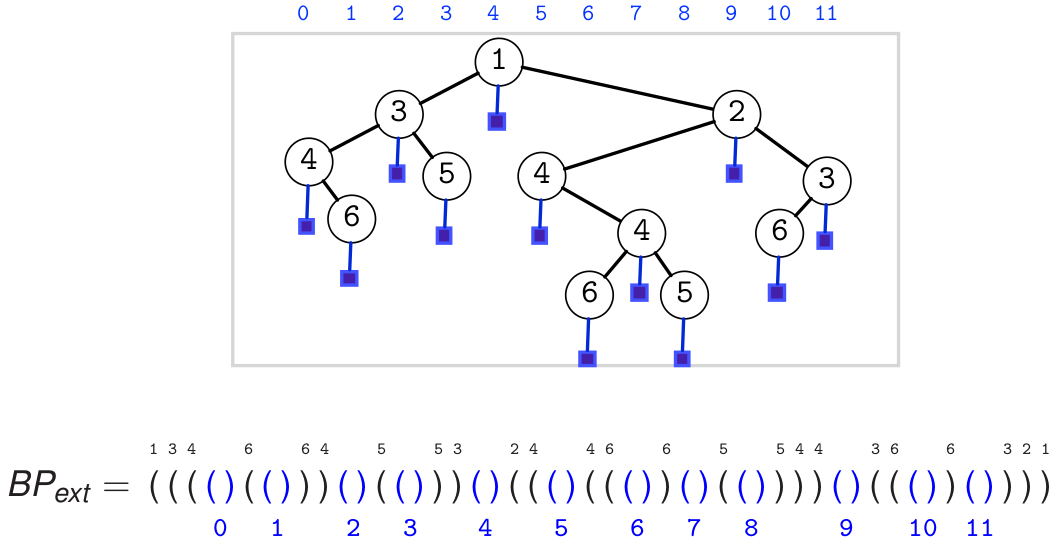
\includegraphics[width=0.8\textwidth]{DFSLCA}
    \captionsetup{width=.8\textwidth}
    \caption{Konstruktion des kartesischen Baums mit Dummy-Blättern (blau) für das Array ``463514645236''. Anschließend wird die Klammernfolge gebildet. In blau hervorgehoben sind die ``Wendepunkte'', also die Dummy-Blätter, und ihr Index}
  \end{figure}

  \item \textbf{RMQ berechnen}. \quad Zur Berechnung von \( \text{rmq}_A(l,r) \) brauchen wir drei Hilfsfunktionen:
  \begin{itemize}
    \item \( \text{rank}(\texttt{pos}, \texttt{char}, \text{BP}_{\text{ext}}) \) gibt die Anzahl an Vorkommisse von \texttt{char} (z.B. ``)'') bis \texttt{pos} in \( \text{BP}_{\text{ext}} \) an.
    \item \( \text{excess}(i) = \text{rank}(i+1, \texttt{(}, \text{BP}_{\text{ext}}) - \text{rank}(i+1, \texttt{)}, \text{BP}_{\text{ext}}) \)
    \item \( \text{select}(j, \texttt{char}, \text{BP}_{\text{ext}}) \) gibt die Position des \( j \)-ten Vorkommens von \texttt{char} in \( \text{BP}_{\text{ext}} \) an.
  \end{itemize}
  Wir können nun den RMQ-Wert folgendermaßen berechnen:

  \begin{pseudocode}
    \textbf{\textsc{rmq}} (A,l,r) \\
    lpos \( \coloneqq \text{select}(l+1, \texttt{()}, \text{BP}_{\text{ext}}) \) \\
    rpos \( \coloneqq \text{select}(r+1, \texttt{()}, \text{BP}_{\text{ext}}) \) \\
    \textbf{return} \( \text{rank} (\text{rmq}^{\pm 1}_{\text{excess}}(\text{lpos}, \text{rpos} + 1), \texttt{()}, \text{BP}_{\text{ext}}) \)
  \end{pseudocode}
\end{itemize}

\subsection{LCA in \( \left\langle O(n),O(1) \right\rangle \) auf \( 2n+o(n) \) Bits}

Die Anzahl an benötigten Bits lässt sich im Vergleich zum vorhergehenden Ansatz noch weiter verkleinern. Wir transformieren dazu den kartesischen Baum --- der ja ein Binärbaum ist --- in einen allgemeinen Baum. Dazu gehen wir folgendermaßen vor:

\begin{enumerate}
  \item Füge einen Elternknoten zur Wurzel des Baums hinzu (der hinzugefügte Knoten ist also die neue Wurzel).
  \item Nehme von jedem Knoten \( v \) --- von der neuen Wurzel ausgehend --- den rechten Kindknoten \( w \), und füge alle Knoten auf dem linkesten Pfad von \( w \) ausgehend zu den Kindknoten von \( v \) hinzu.
\end{enumerate}

\begin{figure}[H]
  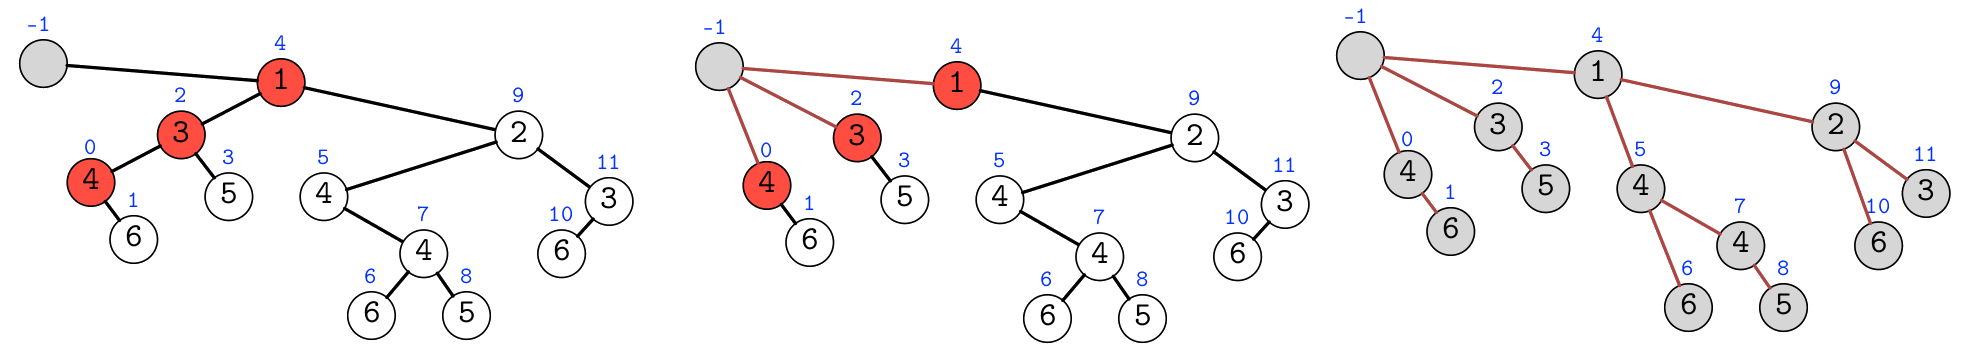
\includegraphics[width=\textwidth]{CartesianTreeTransform}
  \caption{Kartesischer Baum mit neuer Wurzel. Die roten Knoten in der ersten Grafik sind die Knoten, die zu \( v \) --- hier die neue Wurzel --- hinzugefügt werden. Durch Hinzufügen dieser Knoten zu den Kindknoten von \( v \) hat der Baum die Struktur in Grafik 2. Nun wird dieser Prozess rekursiv auf die drei roten Knoten ausgeführt. Ist die Rekursion vollständig abgeschlossen sieht der Baum wie in der dritten Grafik aus}
\end{figure}

Diese Transformation lässt sich bei Bedarf auch rückgängig machen; man kann also, wenn nötig, wieder den Binärbaum konstruieren.

Nun lässt sich wieder die Klammernreihe \( \text{BP} \) von oben bauen. Mit dieser können wir nun RMQ-Abfragen lösen:

\begin{pseudocode}
  \textbf{\textsc{rmq}} (A,l,r) \\
  lpos \( \coloneqq \text{select}(l+2, \texttt{(}, \text{BP}) \) \\
  rpos \( \coloneqq \text{select}(r+2, \texttt{(}, \text{BP}) \) \\
  \textbf{return} \( \text{rank}(\text{rmq}_{\text{excess}}^{\pm 1}(\text{lpos} - 1, \text{rpos}), \texttt{(}, \text{BP}) -1 \)
\end{pseudocode}